\documentclass[12pt,a4paper]{report}

\usepackage[left=2cm, right=2cm, top=4cm, bottom=2cm]{geometry}
\usepackage[utf8x]{inputenc}
\usepackage{fontspec}
\usepackage{enumitem}
\usepackage{amsmath}
\usepackage{tikz}
\usepackage{float}
%\usepackage{pgf}
\usetikzlibrary{arrows,automata}

\usepackage{algpseudocode}
\algblockdefx[Initially]{Initially}{EndInitially}{\textbf{initially do}}{\textbf{end initially}}
\algblockdefx[Upon]{Upon}{EndUpon}[1]{\textbf{upon #1}}{\textbf{end upon}}
\algblockdefx[AsSoon]{AsSoon}{EndAsSoon}[1]{\textbf{as soon as #1}}{\textbf{end as soon}}

\usetikzlibrary{graphs, shapes, graphdrawing}
\usegdlibrary{layered, force}

\begin{document}

	\newcommand{\upon}[1]{\textbf{Upon} #1 \textbf{do}}

	\begin{titlepage}
		\centering
		{\scshape\LARGE Universidad Nacional Autónoma de México \par}
		\vspace{1cm}
		{\scshape\Large Computación Distribuida\par}
		\vspace{1.5cm}
		{\huge\bfseries Tarea 6\par}
		\vspace{.5cm}
		{\Large\itshape Edgar Quiroz Castañeda \par}
	    \vspace{.5cm}
		{\Large\itshape Jerónimo Almeida Rodríguez \par}
		\vfill
		 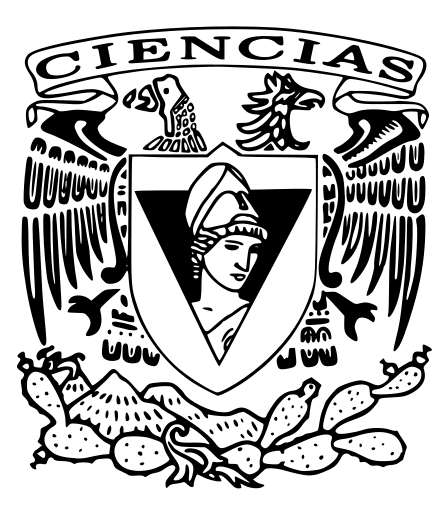
\includegraphics[width=0.5\textwidth]{escudo_f-ciencias.png}
		\vfill

		{\large Jueves 11 de octubre del 2018 \par}
	\end{titlepage}

	\pagebreak
	\setlength{\voffset}{-0.75in}
	\setlength{\headsep}{5pt}

	\begin{enumerate}
		\item {
			Sea $G = (V, E)$ una gráfica. Diseña un algoritmo $BFS$ basado en correr
			$|V|$ instancias del algoritmo $PIF$ cuya complejidad ser
			$O(|E|+|V|\cdot Diam(G))$ en mensajes y $O(Diam(G)^2)$ en tiempo.

			La idea de este algoritmo es recorrer la gráfica por capas por medio de
			una ejecución del $PIF$ por capa.\\
			Cada ejecución tiene el propósito de tomar el árbol de la ejecución
			anterior y agregarle todos los nodos a distancia una más que la ejecución
			anterior.\\
			Para hacer esto, el mensaje que se envía para decubrir son los valores de
			la distancia acumulada y el límite de distancia para esa ejecución en
			particular.\\
			Igualmente que en el otro $BFS$ distribuido, se actualiza la distancia a
			uno más de lo recibido si eso es mejor o igual a lo actual.\\
			Pero sólo se envía esa información a los vecinos en caso de que ellos
			aun estén en el alcance de la ejecución.\\
			Además, si no se es una de las hojas del árbol de la ejecución anterior,
			ni siquiera se envía a todos los vecinos, si no a todos los hijos, que ya
			se conocen desde al menos la ejecución anterior.\\
			En el caso de las hojas del árbol final o de los nodos intermedios del
			árbol de una ejecución dada, se envía la confirmación en cuanto se tiene
			la información de todos los vecinos, .\\
			Para las hojas del árbol de la ejecución, se envía la confirmación en
			cuanto se entera de que es el límite del alcance de esa ejecución.\\
			Como confirmación se envía el conjunto de nodos en su subárbol.\\
			Cuando esto llega a la raíz, es el conjunto de todos los nodos que ya son parte
			del árbol.\\
			Si aun faltan nodos, entonces se aumenta el alcance y se inicia
			una nueva ejecución del $PIF$.
			Si se tiene a todos los nodos en el árbol, entonces el algorítmo acaba.

			\begin{algorithmic}[1]
				\Initially
					\State $children \gets \emptyset$
					\State $acks \gets \emptyset$
					\State $nacks \gets \emptyset$
					\State $discovered \gets \emptyset$
					\If{$p_{id} = root$}
						\State $distance \gets 0$
						\State $parent \gets p_{id}$
						\State $currentBound \gets 1$
						\State send $(distance, currentBound)$ to $neighbors$
					\Else
						\State $parent \gets \bot$
						\State $distance \gets \infty$
					\EndIf
				\EndInitially
				\Statex

				\Upon{receiving $(distance_p, bound)$ from $p$}
					\If{$distance_p + 1 \leq distance$}
						\State $parent \gets p$
						\State $distance \gets distance_p + 1$
					\Else
						\State send $nack$ to $p$
					\EndIf
					\If{$distance -1 < bound $}
						\State send $(distance, bound)$ to $children$
					\ElsIf{$distance -1 = bound $}
						\State send $(distance, bound)$ to $neighbors \setminus \{p\}$
					\ElsIf{$distance = bound$}
						\State send $(ack, discovered)$ to $p$
					\EndIf
				\EndUpon
				\Statex

				\Upon{receiving $(ack, discovered_p)$ from $p$}
					\State $discovered = discovered \cup discovered_p$
					\State $acks = acks \cup \{p\}$
					\State $children = children \cup \{p\}$
				\EndUpon
				\Statex

				\Upon{receiving $nack$ from $p$}
					\State $nacks \gets nacks \cup \{p\}$
				\EndUpon
				\Statex

				\AsSoon{$acks \cup nack = neighbors$}
					\State $acks \gets \emptyset$
					\If{$p_{id} = root$}
						\If{$discovered = V$}
							\State return
						\EndIf
						\If{$acks = children$}
							\State $currentBound \gets currentBound + 1$
							\State send $(distance, currentBound)$ to $neighbors$
						\EndIf
					\Else
						\State send $(ack, discovered)$ to $parent$
					\EndIf
				\EndAsSoon
			\end{algorithmic}
			Con un tiempo normalizado, se tiene que el tiempo para llegar a el nodo $v$
			que está a distancia del diámetro es
			\begin{align*}
				2+4+6+8+...+2\cdot Diam(G) &= 2 (1+2+3+4+...+Diam(G))\\
																	 &= 2\frac{Diam(G)(Diam(G)+1)}{2}\\
																	 &= Diam(G)(Diam(G)+1) \in O(Diam(G)^2)
			\end{align*}
			Pues la ronda $i$ tarda a lo más $2i$ unidades de tiempo, $i$ unidades
			para llegar a el nodo $i$ de la trayectoria de la raíz a $v$, y otras
			$i$ unidades para volver a la raíz.\\
			Este es el último nodo que es agregado al árbol, precisamente porque su
			distancia a la raíz es el diámetro en el peor caso. Entonces este algoritmo
			tiene complejidad en tiepo de $O(Diam(G)^2)$.\\
			En cuanto a la complejidad en mensajes, se tiene que en cada ejecución,
			las aristas que se recorren por primera vez son únicamente las que están
			en el nuevo alcance. Cada una de estas aristas recibe el mensaje con
			la distancia y con el alcance, y devuelve un $ack$ o un $nack$. Como esto
			sólo pasa en la ronda donde son descubiertas, entonces se envían
			$2|E|$ mensajes. Luego, para recorrer el resto de la gráfica hasta
			la raíz se utilizan las trayectorias ya definidas por el subárbol
			descubierto en ejecuciones anterior, que tiene a lo más $|V|-1$ aristas.
			Como este recorrido se hace en cada ejecución, y hay $Diam(G)$ ejecuciones,
			entonces el resto de los mensajes son a los más $(|V|-1)(Diam(G))$.\\
			Entonces, hay a lo más $2|E| + (|V|-1)(Diam(G)) \in O(|E| + |V|Diam(G))$
			mensajes.\\
			Entonces, la complejidad en mensajes es $O(|E| + |V|Diam(G))$.
		}
		\item {
			Explicar por qué el algorítmo Awerbuch $DFS$ tiene complejidad de tiempo
			$O(V)$ ($4|V|-2$) y en mensajes $O(E)$ ($4|E|$). Presentar un ejemplo
			de ejecución en la siguiente gráfica

			Para la complejidad en tiempo, se puede considerar dos fases.
			Primero, cuando un vértice recibe el mensaje que va creando
			el árbol. Le avisa a sus vecinos y espera su confirmación. Esto tarda dos
			unidades de tiempo por cada vértice, es decir $2|V|$. \\
			Además, el mensaje que crea el árbol pasa por todas las aristas de árbol
			dos veces exactamente, una al ser enviado a un nuevo nodo, y otra de
			regreso para confirmar que el árbol en esa parte ya quedó. \\
			Como el árbol tiene $|V|-1$ aristas, esto implica que esa fase tarda
			$2|V|-2$ unidades de tiempo.
			Entonces toma en total $2|V|+2|V|-2 = 4|V|-2 \in O(|V|)$ de tiempo.\\
			Para la complejidad en tiempo, también se pueden considerar dos casos para
			las aristas.\\
			Primero, que una arista $e$ no sea parte del árbol. Entonces ambos de sus
			vértices adyacentes recibieron el mensaje del árbol por alguna otra arista.
			Cuando esto pasó, ambos mandaron un aviso por $e$ y el otro les confirmó
			también por $e$. Esto son cuatro mensajes por cada arista que no esté en
			el árbol.
			Ahora, para alguna arista $(u, v)$ que sí está en el árbol. Cuando el
			mensaje le llegó a $u$, este mandó un aviso a $v$ y esté le confirmó.
			Ahí ya van 2 mensajes. Luego, $u$ le mandó el mensaje del árbol a $v$.
			Eventualmente, cuando el subárbol de $v$ está listo, $v$ le manda un
			aviso de terminado a $u$. Entonces son 4 mensajes por cada arista que sí
			está en el árbol. Entonces son 4 mensajes por arista.
			$4|E| \in O(|E|)$.

			\begin{figure}[H]
				\begin{center}
					\begin{tikzpicture}[node distance = 3cm]
						\begin{scope}[every node/.style = {circle, draw}]
							\node (p1) {$p_1$};
							\node (p2) [above right of = p1] {$p_2$};
							\node (p3) [right of = p2] {$p_3$};
							\node (p4) [below right of = p3] {$p_4$};
							\node (p5) [left of = p4] {$p_4$};
							\node (p6) [below right of = p1] {$p_6$};
						\end{scope}

						\path[-] (p1) edge (p2);
						\path[-] (p1) edge (p5);
						\path[-] (p1) edge (p6);

						\path[-] (p2) edge (p3);
						\path[-] (p2) edge (p4);

						\path[-] (p3) edge (p4);

						\path[-] (p4) edge (p5);
						\path[-] (p4) edge (p6);

						\path[-] (p5) edge (p6);
					\end{tikzpicture}
					\caption{Grafica G}
				\end{center}
			\end{figure}

			\begin{figure}[H]
				\begin{center}
					\begin{tikzpicture}[-,>=stealth',shorten >=1pt,auto,node distance=2.8cm,
						semithick]
						\tikzstyle{every state}=[fill=none,draw=black,text=black]

						\node[label={\tiny $p\leftarrow r$}][state] (A) {$p_1$};
						\node[state] (B) [above right of=A] {$p_2$};
						\node[state] (C) [right of=B] 		{$p_3$};
						\node[state] (D) [below right of=C] {$p_4$};
						\node[state] (E) [below right of=A] {$p_6$};
						\node[state] (F) [above right of=E] {$p_5$};

						\path[->]
						(A) edge[red]		  node  {v} (B)
							edge[red]         node  {v} (F)
							edge[red]		  node  {v} (E);
						\path
						(B) edge 			  node  {} (C)
							edge              node  {} (D)
						(C) edge              node  {} (D)
						(E) edge 			  node  {} (D)
							edge 			  node  {} (F)
						(F) edge 			  node  {} (D);
					\end{tikzpicture}
					\caption{Primer paso del algoritmo. La raíz se autoasigna cómo padre
							 y manda v (visitado) a todos los nodos.}
				\end{center}
			\end{figure}

			\begin{figure}[H]
				\begin{center}
					\begin{tikzpicture}[-,>=stealth',shorten >=1pt,auto,node distance=2.8cm,
						semithick]
						\tikzstyle{every state}=[fill=none,draw=black,text=black]

						\node[label={\tiny $p\leftarrow r$}][state] (A) {$p_1$};
						\node[state] (B) [above right of=A] {$p_2$};
						\node[state] (C) [right of=B] 		{$p_3$};
						\node[state] (D) [below right of=C] {$p_4$};
						\node[state] (E) [below right of=A] {$p_6$};
						\node[state] (F) [above right of=E] {$p_5$};

						\path[<-]
						(A) edge[blue]		  node  {a} (B)
							edge[blue]        node  {a} (F)
							edge[blue]		  node  {a} (E);
						\path
						(B) edge 			  node  {} (C)
							edge              node  {} (D)
						(C) edge              node  {} (D)
						(E) edge 			  node  {} (D)
							edge 			  node  {} (F)
						(F) edge 			  node  {} (D);
					\end{tikzpicture}
					\caption{Los nodos que reciben v devuelven a (ack).}
				\end{center}
			\end{figure}

			\begin{figure}[H]
				\begin{center}
					\begin{tikzpicture}[-,>=stealth',shorten >=1pt,auto,node distance=2.8cm,
						semithick]
						\tikzstyle{every state}=[fill=none,draw=black,text=black]

						\node[label={\tiny $p\leftarrow r$}][state] (A) {$p_1$};
						\node[state] (B) [above right of=A] {$p_2$};
						\node[state] (C) [right of=B] 		{$p_3$};
						\node[state] (D) [below right of=C] {$p_4$};
						\node[state] (E) [below right of=A] {$p_6$};
						\node[state] (F) [above right of=E] {$p_5$};

						\path[->]
						(A) edge[violet]	  node  {t} (B);
						\path
						(A)	edge    	      node  {} (F)
							edge			  node  {} (E)
						(B) edge 			  node  {} (C)
							edge              node  {} (D)
						(C) edge              node  {} (D)
						(E) edge 			  node  {} (D)
							edge 			  node  {} (F)
						(F) edge 			  node  {} (D);
					\end{tikzpicture}
					\caption{La raíz envía t (token) a un nodo.}
				\end{center}
			\end{figure}

			\begin{figure}[H]
				\begin{center}
					\begin{tikzpicture}[-,>=stealth',shorten >=1pt,auto,node distance=2.8cm,
						semithick]
						\tikzstyle{every state}=[fill=none,draw=black,text=black]

						\node[label={\tiny $p\leftarrow r$}][state] (A) {$p_1$};
						\node[label={\tiny $p\leftarrow p_1$}][state][state] (B) [above right of=A] {$p_2$};
						\node[state] (C) [right of=B] 		{$p_3$};
						\node[state] (D) [below right of=C] {$p_4$};
						\node[state] (E) [below right of=A] {$p_6$};
						\node[state] (F) [above right of=E] {$p_5$};

						\path
						(A)	edge    	      node  {} (F)
							edge			  node  {} (E)
						(C) edge              node  {} (D)
						(E) edge 			  node  {} (D)
							edge 			  node  {} (F)
						(F) edge 			  node  {} (D);
						\path[->]
						(B) edge[red]			  node  {v} (C)
							edge[red]              node  {v} (D);
						\path[->]
						(A) edge[violet]		  node  {t} (B);
					\end{tikzpicture}
					\caption{El nodo $p_2$ recibe t, asigna a $p_1$ cómo su padre y envía v
							 a todos sus vecinos.}
				\end{center}
			\end{figure}

			\begin{figure}[H]
				\begin{center}
					\begin{tikzpicture}[-,>=stealth',shorten >=1pt,auto,node distance=2.8cm,
						semithick]
						\tikzstyle{every state}=[fill=none,draw=black,text=black]

						\node[label={\tiny $p\leftarrow r$}][state] (A) {$p_1$};
						\node[label={\tiny $p\leftarrow p_1$}][state][state] (B) [above right of=A] {$p_2$};
						\node[state] (C) [right of=B] 		{$p_3$};
						\node[state] (D) [below right of=C] {$p_4$};
						\node[state] (E) [below right of=A] {$p_6$};
						\node[state] (F) [above right of=E] {$p_5$};

						\path
						(A)	edge    	      node  {} (F)
							edge			  node  {} (E)
						(C) edge              node  {} (D)
						(E) edge 			  node  {} (D)
							edge 			  node  {} (F)
						(F) edge 			  node  {} (D);
						\path[<-]
						(B) edge[blue]			    node  {a} (C)
							edge[blue]              node  {a} (D);
						\path[->]
						(A) edge[violet]			node  {t} (B);
					\end{tikzpicture}
					\caption{Los vecinos de $p_2$ le regresan a.}
				\end{center}
			\end{figure}

			\begin{figure}[H]
				\begin{center}
					\begin{tikzpicture}[-,>=stealth',shorten >=1pt,auto,node distance=2.8cm,
						semithick]
						\tikzstyle{every state}=[fill=none,draw=black,text=black]

						\node[label={\tiny $p\leftarrow r$}][state] (A) {$p_1$};
						\node[label={\tiny $p\leftarrow p_1$}][state] (B) [above right of=A] {$p_2$};
						\node[state] (C) [right of=B]{$p_3$};
						\node[state] (D) [below right of=C] {$p_4$};
						\node[state] (E) [below right of=A] {$p_6$};
						\node[state] (F) [above right of=E] {$p_5$};

						\path
						(A)	edge    	      node  {} (F)
							edge			  node  {} (E)
						(B)	edge              node  {} (D)
						(C) edge              node  {} (D)
						(E) edge 			  node  {} (D)
							edge 			  node  {} (F)
						(F) edge 			  node  {} (D);
						\path[->]
						(B) edge[violet]		    node  {t} (C)
						(A) edge[violet]			node  {t} (B);
					\end{tikzpicture}
					\caption{El nodo $p_2$ envía t, a uno de sus vecinos.}
				\end{center}
			\end{figure}

			\begin{figure}[H]
				\begin{center}
					\begin{tikzpicture}[-,>=stealth',shorten >=1pt,auto,node distance=2.8cm,
						semithick]
						\tikzstyle{every state}=[fill=none,draw=black,text=black]

						\node[label={\tiny $p\leftarrow r$}][state] (A) {$p_1$};
						\node[label={\tiny $p\leftarrow p_1$}][state] (B) [above right of=A] {$p_2$};
						\node[label={\tiny $p\leftarrow p_2$}][state] (C) [right of=B]{$p_3$};
						\node[state] (D) [below right of=C] {$p_4$};
						\node[state] (E) [below right of=A] {$p_6$};
						\node[state] (F) [above right of=E] {$p_5$};

						\path
						(A)	edge    	      node  {} (F)
							edge			  node  {} (E)
						(B)	edge              node  {} (D)
						(E) edge 			  node  {} (D)
							edge 			  node  {} (F)
						(F) edge 			  node  {} (D);
						\path[->]
						(C) edge[red]              node  {v} (D)
						(B) edge[violet]		    node  {t} (C)
						(A) edge[violet]			node  {t} (B);
					\end{tikzpicture}
					\caption{El nodo $p_3$ recibe t, asigna a $p_2$ cómo su padre y envía v
							 a todos sus vecinos.}
				\end{center}
			\end{figure}

			\begin{figure}[H]
				\begin{center}
					\begin{tikzpicture}[-,>=stealth',shorten >=1pt,auto,node distance=2.8cm,
						semithick]
						\tikzstyle{every state}=[fill=none,draw=black,text=black]

						\node[label={\tiny $p\leftarrow r$}][state] (A) {$p_1$};
						\node[label={\tiny $p\leftarrow p_1$}][state] (B) [above right of=A] {$p_2$};
						\node[label={\tiny $p\leftarrow p_2$}][state] (C) [right of=B]{$p_3$};
						\node[state] (D) [below right of=C] {$p_4$};
						\node[state] (E) [below right of=A] {$p_6$};
						\node[state] (F) [above right of=E] {$p_5$};

						\path
						(A)	edge    	      node  {} (F)
							edge			  node  {} (E)
						(B)	edge              node  {} (D)
						(E) edge 			  node  {} (D)
							edge 			  node  {} (F)
						(F) edge 			  node  {} (D);
						\path[<-]
						(C) edge[blue]              node  {a} (D);
						\path[->]
						(B) edge[violet]		    node  {t} (C)
						(A) edge[violet]			node  {t} (B);
					\end{tikzpicture}
					\caption{Los vecinos de $p_3$ le devuelven a.}
				\end{center}
			\end{figure}

			\begin{figure}[H]
				\begin{center}
					\begin{tikzpicture}[-,>=stealth',shorten >=1pt,auto,node distance=2.8cm,
						semithick]
						\tikzstyle{every state}=[fill=none,draw=black,text=black]

						\node[label={\tiny $p\leftarrow r$}][state] (A) {$p_1$};
						\node[label={\tiny $p\leftarrow p_1$}][state] (B) [above right of=A] {$p_2$};
						\node[label={\tiny $p\leftarrow p_2$}][state] (C) [right of=B]{$p_3$};
						\node[state] (D) [below right of=C] {$p_4$};
						\node[state] (E) [below right of=A] {$p_6$};
						\node[state] (F) [above right of=E] {$p_5$};

						\path
						(A)	edge    	      node  {} (F)
							edge			  node  {} (E)
						(B)	edge              node  {} (D)
						(E) edge 			  node  {} (D)
							edge 			  node  {} (F)
						(F) edge 			  node  {} (D);
						\path[->]
						(C) edge[violet]            node  {t} (D)
						(B) edge[violet]		    node  {t} (C)
						(A) edge[violet]			node  {t} (B);
					\end{tikzpicture}
					\caption{El nodo $p_3$ envía t, a uno de sus vecinos.}
				\end{center}
			\end{figure}

			\begin{figure}[H]
				\begin{center}
					\begin{tikzpicture}[-,>=stealth',shorten >=1pt,auto,node distance=2.8cm,
						semithick]
						\tikzstyle{every state}=[fill=none,draw=black,text=black]

						\node[label={\tiny $p\leftarrow r$}][state] (A) {$p_1$};
						\node[label={\tiny $p\leftarrow p_1$}][state] (B) [above right of=A] {$p_2$};
						\node[label={\tiny $p\leftarrow p_2$}][state] (C) [right of=B]{$p_3$};
						\node[label={\tiny $p\leftarrow p_3$}][state] (D) [below right of=C] {$p_4$};
						\node[state] (E) [below right of=A] {$p_6$};
						\node[state] (F) [above right of=E] {$p_5$};

						\path
						(A)	edge    	      node  {} (F)
							edge			  node  {} (E)
						(B)	edge              node  {} (D)
						(E) edge 			  node  {} (D)
							edge			  node  {} (F);
						\path[->]
						(D) edge[red] 			  node  {v} (F)
						(D) edge[red] 			  node  {v} (E)
						(C) edge[violet]            node  {t} (D)
						(B) edge[violet]		    node  {t} (C)
						(A) edge[violet]			node  {t} (B);
					\end{tikzpicture}
					\caption{El nodo $p_4$ recibe t, asigna a $p_3$ cómo su padre y envía v
							 a todos sus vecinos no visitados.}
				\end{center}
			\end{figure}

			\begin{figure}[H]
				\begin{center}
					\begin{tikzpicture}[-,>=stealth',shorten >=1pt,auto,node distance=2.8cm,
						semithick]
						\tikzstyle{every state}=[fill=none,draw=black,text=black]

						\node[label={\tiny $p\leftarrow r$}][state] (A) {$p_1$};
						\node[label={\tiny $p\leftarrow p_1$}][state] (B) [above right of=A] {$p_2$};
						\node[label={\tiny $p\leftarrow p_2$}][state] (C) [right of=B]{$p_3$};
						\node[label={\tiny $p\leftarrow p_3$}][state] (D) [below right of=C] {$p_4$};
						\node[state] (E) [below right of=A] {$p_6$};
						\node[state] (F) [above right of=E] {$p_5$};

						\path
						(A)	edge    	      node  {} (F)
							edge			  node  {} (E)
						(B)	edge              node  {} (D)
						(E) edge 			  node  {} (D)
							edge			  node  {} (F);
						\path[->]
						(E) edge[blue] 			  node  {a} (D)
						(F) edge[blue] 			  node  {a} (D);
						\path[->]
						(C) edge[violet]            node  {t} (D)
						(B) edge[violet]		    node  {t} (C)
						(A) edge[violet]			node  {t} (B);
					\end{tikzpicture}
					\caption{Los vecinos de $p_4$ le devuelven a.	}
				\end{center}
			\end{figure}

			\begin{figure}[H]
				\begin{center}
					\begin{tikzpicture}[-,>=stealth',shorten >=1pt,auto,node distance=2.8cm,
						semithick]
						\tikzstyle{every state}=[fill=none,draw=black,text=black]

						\node[label={\tiny $p\leftarrow r$}][state] (A) {$p_1$};
						\node[label={\tiny $p\leftarrow p_1$}][state] (B) [above right of=A] {$p_2$};
						\node[label={\tiny $p\leftarrow p_2$}][state] (C) [right of=B]{$p_3$};
						\node[label={\tiny $p\leftarrow p_3$}][state] (D) [below right of=C] {$p_4$};
						\node[state] (E) [below right of=A] {$p_6$};
						\node[state] (F) [above right of=E] {$p_5$};

						\path
						(A)	edge    	      node  {} (F)
							edge			  node  {} (E)
						(B)	edge              node  {} (D)
						(E) edge 			  node  {} (F)
						(E) edge 			  node  {} (D);
						\path[->]
						(D) edge[violet] 			node  {t} (F)
						(C) edge[violet]            node  {t} (D)
						(B) edge[violet]		    node  {t} (C)
						(A) edge[violet]			node  {t} (B);
					\end{tikzpicture}
					\caption{El nodo $p_4$ le envía t a algún vecino.}
				\end{center}
			\end{figure}

			\begin{figure}[H]
				\begin{center}
					\begin{tikzpicture}[-,>=stealth',shorten >=1pt,auto,node distance=2.8cm,
						semithick]
						\tikzstyle{every state}=[fill=none,draw=black,text=black]

						\node[label={\tiny $p\leftarrow r$}][state] (A) {$p_1$};
						\node[label={\tiny $p\leftarrow p_1$}][state] (B) [above right of=A] {$p_2$};
						\node[label={\tiny $p\leftarrow p_2$}][state] (C) [right of=B]{$p_3$};
						\node[label={\tiny $p\leftarrow p_3$}][state] (D) [below right of=C] {$p_4$};
						\node[state] (E) [below right of=A] {$p_6$};
						\node[label={\tiny $p\leftarrow p_4$}][state] (F) [above right of=E] {$p_5$};

						\path
						(A)	edge    	      node  {} (F)
							edge			  node  {} (E)
						(B)	edge              node  {} (D)
						(E) edge 			  node  {} (D)
							edge			  node  {} (F)
						(D) edge 			  node  {} (F);
						\path[->]
						(F) edge[red] 			    node  {v} (E)
						(D) edge[violet]            node  {t} (F)
						(C) edge[violet]            node  {t} (D)
						(B) edge[violet]		    node  {t} (C)
						(A) edge[violet]			node  {t} (B);
					\end{tikzpicture}
					\caption{El nodo $p_5$ recibe t, asigna a $p_4$ cómo su padre y envía v
							 a todos sus vecinos no visitados.}
				\end{center}
			\end{figure}

			\begin{figure}[H]
				\begin{center}
					\begin{tikzpicture}[-,>=stealth',shorten >=1pt,auto,node distance=2.8cm,
						semithick]
						\tikzstyle{every state}=[fill=none,draw=black,text=black]

						\node[label={\tiny $p\leftarrow r$}][state] (A) {$p_1$};
						\node[label={\tiny $p\leftarrow p_1$}][state] (B) [above right of=A] {$p_2$};
						\node[label={\tiny $p\leftarrow p_2$}][state] (C) [right of=B]{$p_3$};
						\node[label={\tiny $p\leftarrow p_3$}][state] (D) [below right of=C] {$p_4$};
						\node[state] (E) [below right of=A] {$p_6$};
						\node[label={\tiny $p\leftarrow p_4$}][state] (F) [above right of=E] {$p_5$};

						\path
						(A)	edge    	      node  {} (F)
							edge			  node  {} (E)
						(B)	edge              node  {} (D)
						(E) edge 			  node  {} (D)
							edge			  node  {} (F)
						(D) edge 			  node  {} (F);
						\path[->]
						(E) edge[blue] 			    node  {a} (F)
						(D) edge[violet]            node  {t} (F)
						(C) edge[violet]            node  {t} (D)
						(B) edge[violet]		    node  {t} (C)
						(A) edge[violet]			node  {t} (B);
					\end{tikzpicture}
					\caption{Los vecinos de $p_5$ le devuelven a.}
				\end{center}
			\end{figure}

			\begin{figure}[H]
				\begin{center}
					\begin{tikzpicture}[-,>=stealth',shorten >=1pt,auto,node distance=2.8cm,
						semithick]
						\tikzstyle{every state}=[fill=none,draw=black,text=black]

						\node[label={\tiny $p\leftarrow r$}][state] (A) {$p_1$};
						\node[label={\tiny $p\leftarrow p_1$}][state] (B) [above right of=A] {$p_2$};
						\node[label={\tiny $p\leftarrow p_2$}][state] (C) [right of=B]{$p_3$};
						\node[label={\tiny $p\leftarrow p_3$}][state] (D) [below right of=C] {$p_4$};
						\node[label={\tiny $p\leftarrow p_5$}][state] (E) [below right of=A] {$p_6$};
						\node[label={\tiny $p\leftarrow p_4$}][state] (F) [above right of=E] {$p_5$};

						\path
						(A)	edge    	      node  {} (F)
							edge			  node  {} (E)
						(B)	edge              node  {} (D)
						(E) edge 			  node  {} (D)
							edge			  node  {} (F)
						(D) edge 			  node  {} (F);
						\path[->]
						(F) edge[violet] 			node  {t} (E)
						(D) edge[violet]            node  {t} (F)
						(C) edge[violet]            node  {t} (D)
						(B) edge[violet]		    node  {t} (C)
						(A) edge[violet]			node  {t} (B);
					\end{tikzpicture}
					\caption{El nodo $p_6$ recibe t y asigna a $p_5$ cómo su padre.}
				\end{center}
			\end{figure}

			Cómo en la figura 16, $p_6$ ya no tiene vecinos a quienes enviarle v, tiene que
			devolver el token a su padre. Esto mismo hacen todos los otros nodos hasta llegar
			a la raíz.

			\begin{figure}[H]
				\begin{center}
					\begin{tikzpicture}[-,>=stealth',shorten >=1pt,auto,node distance=2.8cm,
						semithick]
						\tikzstyle{every state}=[fill=none,draw=black,text=black]

						\node[label={\tiny $p\leftarrow r$}][state] (A) {$p_1$};
						\node[label={\tiny $p\leftarrow p_1$}][state] (B) [above right of=A] {$p_2$};
						\node[label={\tiny $p\leftarrow p_2$}][state] (C) [right of=B]{$p_3$};
						\node[label={\tiny $p\leftarrow p_3$}][state] (D) [below right of=C] {$p_4$};
						\node[label={\tiny $p\leftarrow p_5$}][state] (E) [below right of=A] {$p_6$};
						\node[label={\tiny $p\leftarrow p_4$}][state] (F) [above right of=E] {$p_5$};

						\path
						(A)	edge    	      node  {} (F)
							edge			  node  {} (E)
						(B)	edge              node  {} (D)
						(E) edge 			  node  {} (D)
							edge			  node  {} (F)
						(D) edge 			  node  {} (F);
						\path[<-]
						(F) edge[violet] 			node  {$t_0$} (E)
						(D) edge[violet]            node  {$t_1$} (F)
						(C) edge[violet]            node  {$t_2$} (D)
						(B) edge[violet]		    node  {$t_3$} (C)
						(A) edge[violet]			node  {$t_4$} (B);
					\end{tikzpicture}
					\caption{El token regresa hasta la raíz.}
				\end{center}
			\end{figure}

			\begin{figure}[H]
				\begin{center}
					\begin{tikzpicture}[-,>=stealth',shorten >=1pt,auto,node distance=2.8cm,
						semithick]
						\tikzstyle{every state}=[fill=none,draw=black,text=black]

						\node[label={\tiny $p\leftarrow r$}][state] (A) {$p_1$};
						\node[label={\tiny $p\leftarrow p_1$}][state] (B) [above right of=A] {$p_2$};
						\node[label={\tiny $p\leftarrow p_2$}][state] (C) [right of=B]{$p_3$};
						\node[label={\tiny $p\leftarrow p_3$}][state] (D) [below right of=C] {$p_4$};
						\node[label={\tiny $p\leftarrow p_5$}][state] (E) [below right of=A] {$p_6$};
						\node[label={\tiny $p\leftarrow p_4$}][state] (F) [above right of=E] {$p_5$};

						\path
						(F) edge[violet] 			node  {} (E)
						(D) edge[violet]            node  {} (F)
						(C) edge[violet]            node  {} (D)
						(B) edge[violet]		    node  {} (C)
						(A) edge[violet]			node  {} (B);
					\end{tikzpicture}
					\caption{Árbol formado al final de la ejecución del algoritmo.}
				\end{center}
			\end{figure}

		}

		\item {
			Ver el video y mediante una lista de puntos explicar las ideas que se
			exponon. Cada punto no debe tener más de un par de líneas.
			The Physics and Philosophy of Time - with Carlo Rovelli https://youtu.be/-6rWqJhDv7M

			Nuestras experiencias son una secuencia de momentos en una dirección,
			el pasado está dado; tenemos regitros y estudios de él, deja rastros y
			memorias.
			El tiempo es un paquete de propiedades combinadas que si se separan,
			no queda nada. La implicación de las tres juntas forma algo muy fuerte.
			Aunque según
			nuestra percepción, el tiempo transcurre de la misma manera para todos.
			La linea de tiempo no es acertada, pues el tiempo no es fijo
			para todo en el universo.\\
			Uno sabe su definición de "ahora", pero no puedo decir que ahora veo algo;
			veo la versión del tiempo que tarda en llegar eso a mí. Entonces, no hay
			definición de ahora mas que restringida al tiempo en que tarda en ir y
			venir la luz. Así, se puede definir el ahora cómo $c\cdot\Delta t$
			Fuera de este radio, no hay un "ahora" objetivo. Existe
			una serie de eventos relacionados entre sí, pero no con un orden
			matemático.\\
			Ayer está fijo y lo conocemos, mañana no sabemos; pero para todas las
			ecuaciones fundamentales de física no hay distinción entre el presente y el
			futuro. La entropía, entonces no es solamente una cantidad fundamental,
			sino también manera en la que las cosas están desordenadas. Este orden
			esta dado por el observador, no por las cosas en sí. Entonces, la entropía está
			dada segun la descripción del sistema y depende de la manera en la que se
			interactúa con el sistema. Así, la distinción entre el pasado y el futuro
			es el orden en el pasado que no encontramos en el futuro.
			Sin entropía (desorden) no tendríamos estos rastros del
			pasado, no habría marca de lo que sucedió. Es el orden mayor del pasado
			que da cabida al desorden que marca los sucesos.\\
			Cómo el reloj es un objeto cuántico, puede estar en una superposición. Así,
			toda nuestra percepción actual del tiempo desaparece en perspectiva de la
			gravedad cuántica. A un nivel básico, el tiempo es una cuenta de cambios,
			según Aristóteles. Kant, por otro lado propone que es algo que fluye
			uniformemente independientemente de que haya o no cambios. Einstein propone
			que son objetos dinámicos, un campo gravitacional.\\
			Si la
			velocidad de la luz es infinita, entonces podemos hablar en términos de
			un mismo momento.\\
			La baja entropía del pasado no es entonces por su origen sino por la
			perspectiva que nosotros tenemos de él. Así, el flujo del tiempo no está
			descrito por las leyes de la física sino por nuestra percepción.
			La linea del tiempo es una metáfora para nuestras memorias del pasado y lo
			que anticipamos para el futuro. Nosotros somos la máquina del tiempo, no
			el universo.\\
			El tiempo no es neutral para nosotros. El impulso del cerebro que controla
			nuestra manera de interactuar está orientada en el tiempo. El tiempo, para
			nosotros es la conección emocional a los eventos que fluyen, que están en
			el pasado. El tiempo es todas estas capas que se generan desde nosotros.
			Afuera de estas capas, solamente existe una vaga forma de temporalidad.
			De esta manera, el tiempo es toda esta relación de las emociones que
			hemos relacionado.
		}
	\end{enumerate}
\end{document}
